\documentclass{article}
\usepackage{amsmath}
\usepackage[utf8]{inputenc}
\usepackage{graphicx}
\usepackage{verbatim}
\usepackage{float}
\usepackage[makeroom]{cancel}
\usepackage[english]{babel}
\usepackage{textcomp}
\usepackage{gensymb}
\usepackage{color}
\usepackage{subcaption}
\usepackage{caption}
\usepackage{hyperref}
\usepackage{physics}
\usepackage{dsfont}
%\usepackage{amsfonts}
\usepackage{listings}
\usepackage{multicol}
\usepackage{units}

% From Eirik's .tex
\usepackage{epstopdf}
\usepackage{cite}
\usepackage{braket}
\usepackage{url}
\bibliographystyle{plain}

\usepackage{algorithmicx}
\usepackage{algorithm}% http://ctan.org/pkg/algorithms
\usepackage{algpseudocode}% http://ctan.org/pkg/algorithmicx

\usepackage[margin=1cm]{caption}
\usepackage[outer=1.2in,inner=1.2in]{geometry}
% For writing full-size pages
%\usepackage{geometry}
%\geometry{
%  left=5mm,
%  right=5mm,
%  top=5mm,
%  bottom=5mm,
%  heightrounded,
%}

% Finding overfull \hbox
\overfullrule=2cm

\lstset{language=IDL}
 %\lstset{alsolanguage=c++}
\lstset{basicstyle=\ttfamily\small}
 %\lstset{backgroundcolor=\color{white}}
\lstset{frame=single}
\lstset{stringstyle=\ttfamily}
\lstset{keywordstyle=\color{red}\bfseries}
\lstset{commentstyle=\itshape\color{blue}}
\lstset{showspaces=false}
\lstset{showstringspaces=false}
\lstset{showtabs=false}
\lstset{breaklines}
\lstset{aboveskip=20pt,belowskip=20pt}

\lstset{basicstyle=\footnotesize, basewidth=0.5em}
\lstdefinestyle{cl}{frame=none,basicstyle=\ttfamily\small}
\lstdefinestyle{pr}{frame=single,basicstyle=\ttfamily\small}
\lstdefinestyle{prt}{frame=none,basicstyle=\ttfamily\small}
% \lstinputlisting[language=Python]{filename}


\definecolor{codepurple}{rgb}{0.58,0,0.82}
\definecolor{backcolour}{rgb}{0.95,0.95,0.92}
\definecolor{dkgreen}{rgb}{0,0.6,0}
\definecolor{gray}{rgb}{0.5,0.5,0.5}
\definecolor{magenta}{rgb}{0.58,0,0.82}

\lstdefinestyle{pystyle}{
  language=Python,
  aboveskip=3mm,
  belowskip=3mm,
  columns=flexible,
  basicstyle={\small\ttfamily},
  backgroundcolor=\color{backcolour},
  commentstyle=\color{dkgreen},
  keywordstyle=\color{magenta},
  numberstyle=\tiny\color{gray},
  stringstyle=\color{codepurple},
  basicstyle=\footnotesize,
  breakatwhitespace=false,
  breaklines=true,
  captionpos=b,
  keepspaces=true,
  numbers=left,
  numbersep=5pt,
  showspaces=false,
  showstringspaces=false,
  showtabs=false,
  tabsize=2
}

%%%%%%%%%%%%%%%%%%%%%%%%%%%%%%%%
% Self made macros here yaaaaaay
\newcommand\answer[1]{\underline{\underline{#1}}}
\newcommand\pd[2]{\frac{\partial #1}{\partial #2}}
\newcommand\red[1]{\textcolor{red}{\textbf{#1}}}
\newcommand\numberthis{\addtocounter{equation}{1}\tag{\theequation}}
% Usage: \numberthis \label{name}
% Referencing: \eqref{name}

% Some matrices
\newcommand\smat[1]{\big(\begin{smallmatrix}#1\end{smallmatrix}\big)}
\newcommand\ppmat[1]{\begin{pmatrix}#1\end{pmatrix}}

% Section labeling
\usepackage{titlesec}% http://ctan.org/pkg/titlesec
\renewcommand{\thesubsection}{\arabic{subsection}}


% Title/name/date
\title{FYS4150 - Project 2}
\author{Simen Nyhus Bastnes \& Eirik Ramsli Hauge}
\date{3. October 2016}

\begin{document}
\maketitle

\begin{abstract}
Wow dude, so this is like, so abstract dude. Have you ever had a dream that you, um, you had, your, you- you could, you’ll do, you- you wants, you, you could do so, you- you’ll do, you could- you, you want, you want them to do you so much you could do anything?
\end{abstract}
\subsection{Introduction}
In project 2, we aim to solve Schrödinger's equation for two electrons with and without a repulsive Coulomb interaction in a three-dimensional harmonic oscillator well. We start by reformulating the equation in a discretized form as an eigenvalue equation, which can be solved with Jacobi's method. \\\\We can then compare our implementation Jacobi's method fares against ``smarter'' algorithms for solving eigenvalue equations. Finally, we will look at implementing unit-tests, in order to test that the various parts of our program does what it's intended to do.\\\\
\red{Should maybe be rewritten, or changed order, or add more, dunno}
\subsection{Theory}
\subsubsection{Schrödinger's equation}
In this project, we will assume that the electrons move in a three-dimensional harmonic oscillator potential, and repel each other via the static Coulomb interaction. By assuming spherical symmetry, the solution for the radial part of Schrödinger's equation for one electron reads
\begin{align*}
  -\frac{\hbar^2}{2m}\bigg(\frac{1}{r^2}\frac{d}{dr}r^2\frac{d}{dr} - \frac{l(l+1)}{r^2}\bigg)R(r) + V(r)R(r) = ER(r)\numberthis\label{eq:radial_schroedinger}
\end{align*}
For the rest of the project, we set the orbital momentum quantum number $l$ to zero. In our non-interacting case, the harmonic oscillator potential $V(r) = (1/2)kr^2$ with $k=m\omega^2$.\\\\We perform a substitution for $R(r) = (1/r)u(r)$, introduce a dimensionless variable $\rho = (1/\alpha)r$, where $\alpha$ is a constant with dimension length $\alpha = (\hbar^2/mk)^{1/4}$. Inserting this into the Scrödinger equation \eqref{eq:radial_schroedinger}, we get
\begin{align*}
-\frac{d^2}{d\rho^2}u(\rho) + \rho^2u(\rho) = \lambda u(\rho)\numberthis\label{eq:dimless_schroedinger}
\end{align*}
where $\lambda = (2m\alpha^2/\hbar^2)E$. Equation \eqref{eq:dimless_schroedinger} is the first equation we want to solve numerically, and we will later use that for $l=0$, the first eigenvalues $\lambda$ are $\lambda_0 = 3$, $\lambda_1 = 7$ and $\lambda_2 = 11$.\\\\
Starting our journey to write equation \eqref{eq:dimless_schroedinger} as an eigenvalue equation, we use the by now standard expression for the second derivative
\begin{align*}
  u'' = \frac{u(\rho+h)-2u(\rho)+u(\rho-h)}{h^2}+\mathcal{O}(h^2)
\end{align*}
where $h$ is our step length. We define minimum and maximum values for $\rho$, $\rho_{\text{min}} = 0$ and $\rho_{\text{max}}$, as we cannot set $\rho_{\text{max}} = \infty$. When setting $\rho_{\text{max}}$, we need to make sure that it is set high enough so that the square of the wavefunction $u$ is small near $\rho_{\text{max}}$ for accuracy of the solution. Next, we split this interval into $N$ number of mesh points, so that we can define the step length as
\begin{align*}
  h = \frac{\rho_N-\rho_0}{N}
\end{align*}
where $\rho_0 = \rho_{\text{min}}$ and $\rho_{\text{max}} =\rho_N$. This gives us an expression for $\rho$ at point $i$
\begin{align*}
  \rho_i = \rho_0 + ih\;\;\;\;\;\;\;\;\;i=1,2,\dots,N
\end{align*}
Now we can rewrite the second derivative as
\begin{align*}
  u_i'' = \frac{u_{i+1}-2u_i + u_{i-1}}{h^2}
\end{align*}
Using this, we can rewrite the dimensionless Schrödinger equation \eqref{eq:dimless_schroedinger} as a discretized equation.
\begin{align*}
  -\frac{u_{i+1}-2u_i+u_{i-1}}{h^2} + \rho_i^2u_i = -\frac{u_{i+1}-2u_i+u_{i-1}}{h^2} + V_iu_i = \lambda u_i \numberthis\label{eq:discretized_schroedinger}
\end{align*}
where $V_i = \rho_i^2$ is the harmonic oscillator potential. From the previous project, we recall that we can represent equation \eqref{eq:discretized_schroedinger} in terms of a tridiagonal matrix, where the diagonal elements are given by
\begin{align*}
  d_i = \frac{2}{h^2} + V_i = \frac{2}{h^2} + \rho_i^2
\end{align*}
and the non-diagonal matrix elements
\begin{align*}
  e_i = -\frac{1}{h^2}
\end{align*}
We notice that in this case, the non-diagonal matrix elements are constant. Using this, we can now write the Schrödinger equation as
\begin{align*}
  d_iu_i + e_{i-1}u_{i-1} + e_{i+1}u_{i+1} = \lambda u_i
\end{align*}
So that we now have the following eigenvalue equation
\begin{align*}
\ppmat{\frac{2}{h^2}+V_1&-\frac{1}{h^2}&0&\dots&0\\
    -\frac{1}{h^2}&\frac{2}{h^2}+V_2&-\frac{1}{h^2}&0&\dots\\
    \dots&\dots&\dots&\dots&0\\
    \dots&\dots&-\frac{1}{h^2}&\frac{2}{h^2}+V_{N-2}&-\frac{1}{h^2}\\
    0&\dots&0&-\frac{1}{h^2}&\frac{2}{h^2}+V_{N-1}}
  \ppmat{u_1\\u_2\\\dots\\u_{N-2}\\u_{N-1}} = \lambda
  \ppmat{u_1\\u_2\\\dots\\u_{N-2}\\u_{N-1}} \numberthis\label{eq:eigval_eq}
\end{align*}
which is what we want to solve by using Jacobi's method.
\subsubsection*{Interacting case}
The eigenvalue equation \eqref{eq:eigval_eq} was derived by assuming one electron in a harmonic oscillator potential. For two electrons with no repulsive Coulomb interaction, we have the following Schrödinger equation
\begin{align*}
  \bigg(-\frac{\hbar^2}{2m}\frac{d^2}{dr_1^2} - \frac{\hbar^2}{2m}\frac{d^2}{dr_2^2} + \frac{1}{2}kr_1^2 + \frac{1}{2}kr_2^2\bigg)u(r_1,r_2) = E^{(2)}u(r_1,r_2)
\end{align*}
With no interaction, this can be written out as the product of two single-electron wave functions, like we did earlier. Introducing relative coordinates $\mathbf{r} = \mathbf{r_1} - \mathbf{r_2}$ and center-of-mass coordinate $\mathbf{R} = 1/2(\mathbf{r_1}+\mathbf{r_2})$, and adding the repulsive Coulomb interaction between the two electrons to our potential
\begin{align*}
  V(r_1,r_2) = \frac{\beta e^2}{|\mathbf{r_1}-\mathbf{r_2}|} = \frac{\beta e^2}{r}
\end{align*}
So that we get the following radial Schrödinger equation (omitting the center-of-mass motion)
\begin{align*}
  \bigg(-\frac{\hbar^2}{m}\frac{d^2}{dr^2} + \frac{1}{4}kr^2 + \frac{\beta e^2}{r}\bigg)\psi(r) = E_r\psi(r)\\
\end{align*}
This is quite similar to the equation \eqref{eq:radial_schroedinger} we found earlier, and we can likewise introduce a dimensionless variable $\rho = r/\alpha$, and rewrite Schrödinger's equation as
\begin{align*}
  -\frac{d^2}{d\rho^2}\psi(\rho) + \omega_r^2\rho^2\psi(\rho) + \frac{1}{\rho}\psi(\rho) = \lambda\psi(\rho)
\end{align*}
So we see that the only thing we have to modify when adding the repulsive coloumb interaction is to change the potential from $\rho^2$ to $\omega_r\rho^2 + 1/\rho$, where we treat $\omega_r$ as a parameter reflecting the strength of the harmonic oscillator potential. We will later look at how the wave function behaves for different values of $\omega_r$.
\subsubsection{Jacobi's method}
\subsection{Experimental}
The programs used in this project can be found in the GitHub repository \cite{Github}, in the \texttt{/src/} folder. When running the program, it takes 3 command line arguments, $N$, $\rho_{\text{max}}$ and \texttt{mode}. The program has three different runmodes, which we will discuss in some more detail. The text-files saved by the program lies in the \texttt{/benchmarks/} folder, while plots are in \texttt{/figures/}.
\subsubsection{Non-interacting case}
Setting \texttt{mode} to \texttt{non-interact} runs the program with specified dimension and $\rho_{\text{max}}$, and stores the 5 lowest eigenvalues (calculated both by Jacobi's method and Armadillo's \texttt{eig\_sym()} function) in a file \texttt{eigenvalues\_noint\_n<N>.dat}. The execution time for both methods are appended to the file \texttt{timing.txt}.
\subsubsection{Interacting case}
Setting \texttt{mode} to \texttt{interact} runs the program for 4 different values of $\omega_r$ (0.01, 0.5, 1.0, 5.0) with the Coulomb interaction added.\\The eigenvector for the ground state is written to the file \texttt{eigenvectors\_int\_n<N>.dat}
\subsubsection{Unit tests}
Setting \texttt{mode} to \texttt{unit\_tests} runs three unit tests on the different modules in our program, and the result from the tests is written to the file \texttt{unittest.txt}.
\\\\\red{add the different unit tests, and what they do}
\subsection{Results}
\begin{figure}[H]
  \centering
  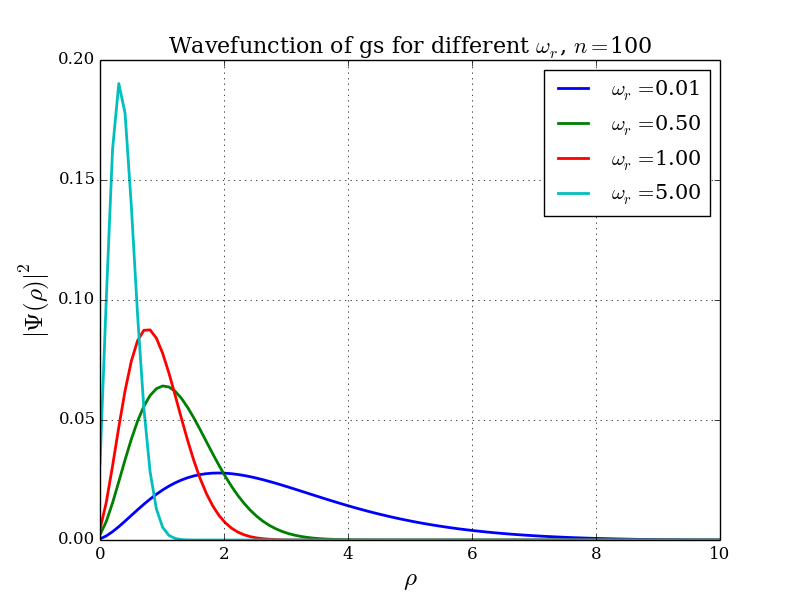
\includegraphics[scale=0.5]{../figures/eigvec_interact_n100.png}
  \caption{Plot of the eigenvectors for the interacting case for $n=100$}
  \label{fig:eigvec100}
\end{figure}
\subsection{Discussion}

\subsection{Conclusion}
\bibliography{references}
\end{document}
